\documentclass[a4paper, 14pt]{extarticle}

% Поля
%--------------------------------------
\usepackage{geometry}
\geometry{a4paper,tmargin=2cm,bmargin=2cm,lmargin=3cm,rmargin=1cm}
%--------------------------------------


%Russian-specific packages
%--------------------------------------
\usepackage[T2A]{fontenc}
\usepackage[utf8]{inputenc} 
\usepackage[english, main=russian]{babel}
%--------------------------------------

\usepackage{textcomp}

% Красная строка
%--------------------------------------
\usepackage{indentfirst}               
%--------------------------------------             


%Graphics
%--------------------------------------
\usepackage{graphicx}
\graphicspath{ {./images/} }
\usepackage{wrapfig}
%--------------------------------------

% Полуторный интервал
%--------------------------------------
\linespread{1.3}                    
%--------------------------------------

%Выравнивание и переносы
%--------------------------------------
% Избавляемся от переполнений
\sloppy
% Запрещаем разрыв страницы после первой строки абзаца
\clubpenalty=10000
% Запрещаем разрыв страницы после последней строки абзаца
\widowpenalty=10000
%--------------------------------------

%Списки
\usepackage{enumitem}

%Подписи
\usepackage{caption} 

%Гиперссылки
\usepackage{hyperref}

\hypersetup {
	unicode=true
}

%Рисунки
%--------------------------------------
\DeclareCaptionLabelSeparator*{emdash}{~--- }
\captionsetup[figure]{labelsep=emdash,font=onehalfspacing,position=bottom}
%--------------------------------------

\usepackage{tempora}

%Листинги
%--------------------------------------
\usepackage{listings}
\lstset{
  basicstyle=\ttfamily\footnotesize, 
  %basicstyle=\footnotesize\AnkaCoder,        % the size of the fonts that are used for the code
  breakatwhitespace=false,         % sets if automatic breaks shoulbd only happen at whitespace
  breaklines=true,                 % sets automatic line breaking
  captionpos=t,                    % sets the caption-position to bottom
  inputencoding=utf8,
  frame=single,                    % adds a frame around the code
  keepspaces=true,                 % keeps spaces in text, useful for keeping indentation of code (possibly needs columns=flexible)
  keywordstyle=\bf,       % keyword style
  numbers=left,                    % where to put the line-numbers; possible values are (none, left, right)
  numbersep=5pt,                   % how far the line-numbers are from the code
  xleftmargin=25pt,
  xrightmargin=25pt,
  showspaces=false,                % show spaces everywhere adding particular underscores; it overrides 'showstringspaces'
  showstringspaces=false,          % underline spaces within strings only
  showtabs=false,                  % show tabs within strings adding particular underscores
  stepnumber=1,                    % the step between two line-numbers. If it's 1, each line will be numbered
  tabsize=2,                       % sets default tabsize to 8 spaces
  title=\lstname                   % show the filename of files included with \lstinputlisting; also try caption instead of title
}
%--------------------------------------

%%% Математические пакеты %%%
%--------------------------------------
\usepackage{amsthm,amsfonts,amsmath,amssymb,amscd}  % Математические дополнения от AMS
\usepackage{mathtools}                              % Добавляет окружение multlined
\usepackage[perpage]{footmisc}
%--------------------------------------

%--------------------------------------
%			НАЧАЛО ДОКУМЕНТА
%--------------------------------------

\begin{document}

%--------------------------------------
%			ТИТУЛЬНЫЙ ЛИСТ
%--------------------------------------
\begin{titlepage}
\thispagestyle{empty}
\newpage


%Шапка титульного листа
%--------------------------------------
\vspace*{-60pt}
\hspace{-65pt}
\begin{minipage}{0.3\textwidth}
\hspace*{-20pt}\centering

\includegraphics[width=\textwidth]{emblem}
\end{minipage}
\begin{minipage}{0.67\textwidth}\small \textbf{
\vspace*{-0.7ex}
\hspace*{-6pt}\centerline{Министерство науки и высшего образования Российской Федерации}
\vspace*{-0.7ex}
\centerline{Федеральное государственное бюджетное образовательное учреждение }
\vspace*{-0.7ex}
\centerline{высшего образования}
\vspace*{-0.7ex}
\centerline{<<Московский государственный технический университет}
\vspace*{-0.7ex}
\centerline{имени Н.Э. Баумана}
\vspace*{-0.7ex}
\centerline{(национальный исследовательский университет)>>}
\vspace*{-0.7ex}
\centerline{(МГТУ им. Н.Э. Баумана)}}
\end{minipage}
%--------------------------------------

%Полосы
%--------------------------------------
\vspace{-25pt}
\hspace{-35pt}\rule{\textwidth}{2.3pt}

\vspace*{-20.3pt}
\hspace{-35pt}\rule{\textwidth}{0.4pt}
%--------------------------------------

\vspace{1.5ex}
\hspace{-35pt} \noindent \small ФАКУЛЬТЕТ\hspace{80pt} <<Информатика и системы управления>>

\vspace*{-16pt}
\hspace{47pt}\rule{0.83\textwidth}{0.4pt}

\vspace{0.5ex}
\hspace{-35pt} \noindent \small КАФЕДРА\hspace{50pt} <<Теоретическая информатика и компьютерные технологии>>

\vspace*{-16pt}
\hspace{30pt}\rule{0.866\textwidth}{0.4pt}
  
\vspace{11em}

\begin{center}
\Large {\bf Летучка № 1} \\
\large {\bf по курсу <<Численные методы линейной алгебры>>} \\
\large <<Реализация метода прогонки и оценка погрешности вычислений>>
\end{center}\normalsize

\vspace{8em}


\begin{flushright}
  {Студентка группы ИУ9-72Б Самохвалова П. С. \hspace*{15pt}\\
  \vspace{2ex}
  Преподаватель Посевин Д. П.\hspace*{15pt}}
\end{flushright}

\bigskip

\vfill
 

\begin{center}
\textsl{Москва 2023}
\end{center}
\end{titlepage}
%--------------------------------------
%		КОНЕЦ ТИТУЛЬНОГО ЛИСТА
%--------------------------------------

\renewcommand{\ttdefault}{pcr}

\setlength{\tabcolsep}{3pt}
\newpage
\setcounter{page}{2}

\section{Цель}\label{Sect::goal}

Реализовать метод прогонки и оценить его погрешность в сравнении с простейшим методом Гаусса и библиотечным решением.

\section{Задание}\label{Sect::task}

\begin{enumerate}
    \item Реализовать метод прогонки для Ax = f, A $ \in R^{100×100}$, f, x $ \in R^{100}$, A - трехдиагональная матрица.
    \item Найти относительные погрешности метода прогонки, метода Гаусса и библиотечного метода и сравнить их.
\end{enumerate}

\section{Практическая реализация}\label{Sect::code}

Исходный код программы представлен в листинге~\ref{lst:code1}.   

\begin{lstlisting}[language={python},caption={Метод прогонки},label={lst:code1}]
import copy
import random
from num_methods import *
import numpy as np


def progonka_method(m, d):
    n = len(m)
    a = [0]
    b = [0]
    c = [0]
    for i in range(n):
        for j in range(n):
            if i == j:
                b.append(m[i][j])
            elif i == j + 1:
                a.append(m[i][j])
            elif i == j - 1:
                c.append(m[i][j])
    d = [0] + d
    alpha = [0] * n
    beta = [0] * n
    for i in range(1, n):
        alpha[i] = -c[i] / (a[i - 1] * alpha[i - 1] + b[i])
        beta[i] = (d[i] - a[i - 1] * beta[i - 1]) / (a[i - 1] * alpha[i - 1] + b[i])
    x = [0] * (n + 1)
    x[n] = (d[n] - a[n - 1] * beta[n - 1]) / (a[n - 1] * alpha[n - 1] + b[n])
    for i in range(n - 1, 0, -1):
        x[i] = alpha[i] * x[i + 1] + beta[i]
    x = x[1:]
    return x


def gauss_method(a, b):
    n = len(a)
    for i in range(n):
        for j in range(i + 1, n):
            c = - a[j][i] / a[i][i]
            for k in range(i, n):
                if k == i:
                    a[j][k] = 0
                else:
                    a[j][k] += c * a[i][k]
            b[j] += c * b[i]
    x = [0] * n
    for i in range(n - 1, -1, -1):
        x[i] = b[i]
        for j in range(n - 1, i, -1):
            x[i] -= x[j] * a[i][j]
        x[i] /= a[i][i]
    return x


def generate_tridiagonal_matrix(n, v1, v2):
    a = [[0] * n for i in range(n)]
    for i in range(n):
        if i == 0:
            a[i][i] = random.uniform(v1, v2)
            a[i][i + 1] = random.uniform(v1, v2)
        elif i == n - 1:
            a[i][i] = random.uniform(v1, v2)
            a[i][i - 1] = random.uniform(v1, v2)
        else:
            a[i][i] = random.uniform(v1, v2)
            a[i][i - 1] = random.uniform(v1, v2)
            a[i][i + 1] = random.uniform(v1, v2)
    return a


n = 100
v1 = -100
v2 = 100
a = generate_tridiagonal_matrix(n, v1, v2)
x = [random.uniform(v1, v2) for i in range(1, n + 1)]
b = mult_matr_vec(a, x)

x1 = gauss_method(copy.deepcopy(a), copy.deepcopy(b))
print("Gauss method")
print(norm_vec(sub_vec(x, x1)) * 100)
print()

x2 = progonka_method(copy.deepcopy(a), copy.deepcopy(b))
print("Progonka method")
print(norm_vec(sub_vec(x, x2)) * 100)
print()

x3 = np.linalg.solve(a, b)
print("Library method")
print(norm_vec(sub_vec(x, x3)) * 100)
print()

\end{lstlisting}

\section{Результаты}\label{Sect::res}

Результаты работы программы представлены на рисунке~\ref{fig:img1}.

\begin{figure}[!htb]
	\centering
	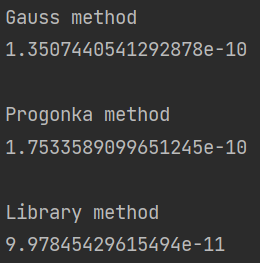
\includegraphics[width=0.8\textwidth]{img1}
\caption{Результаты}
\label{fig:img1}
\end{figure}

\section{Выводы}\label{Sect::conclusion}

В результате выполнения лабораторной работы был реализован метод прогонки, было проведено сравнение точности решения методом прогонки, методом Гаусса и библиотечным методом.

\end{document}
